%--------------------------------------------------------------------
%--------------------------------------------------------------------
% Formato para los talleres del curso de Métodos Computacionales
% Universidad de los Andes
%--------------------------------------------------------------------
%--------------------------------------------------------------------

\documentclass[11pt]{article}
\usepackage[utf8]{inputenc}
\usepackage{graphicx}
\usepackage{tabularx}
\usepackage[absolute]{textpos} % Para poner una imagen en posiciones arbitrarias
\usepackage{multirow}
\usepackage{float}
\usepackage{hyperref}
%\decimalpoint

\begin{document}
\begin{center}
{\Large Métodos Computacionales} \\
S4C4 - \textsc{Makefile}\\
07-2018\\
\end{center}


\noindent
\section{Gr\'aficas}
\begin{center}
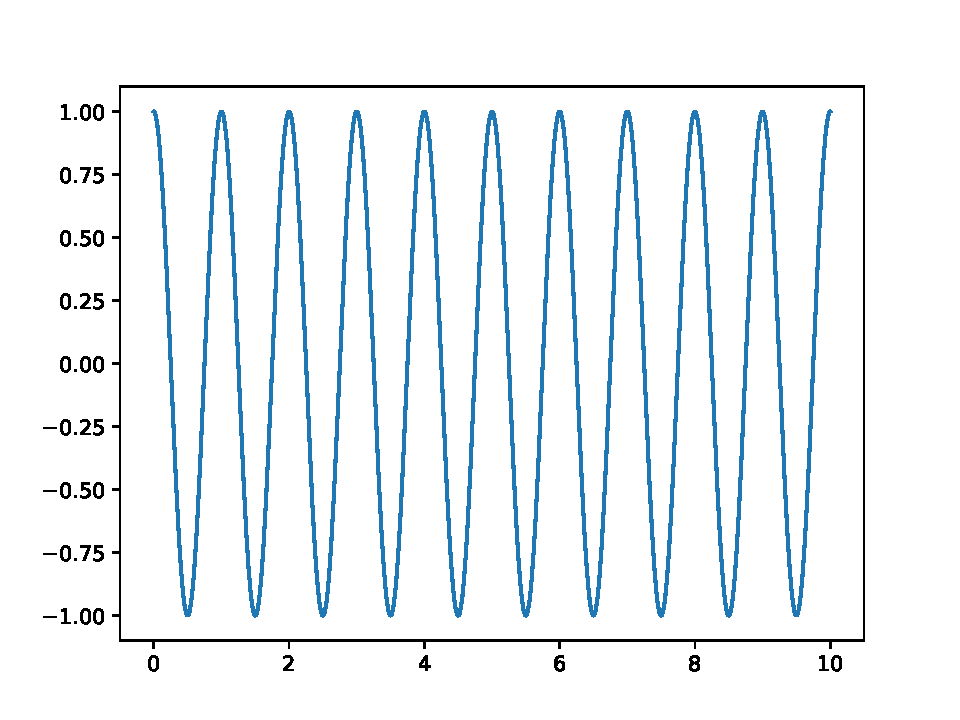
\includegraphics[width=10cm]{plot.pdf} 
\begin{center}
\end{center}
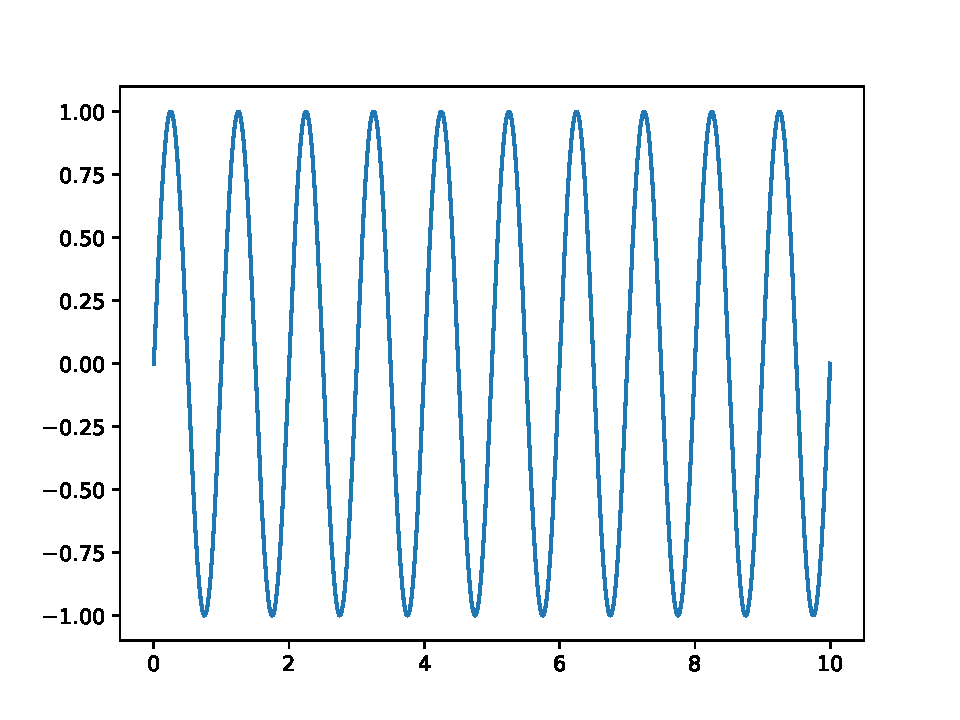
\includegraphics[width=10cm]{plot1.pdf} 
\end{center}


\end{document}
